\section{Line-following Robot}
\label{sec:linefollwerrobot}
%\fbox{LIU: OpenModelica Sensors not available.}

\subsection{Example Description}

This example, originally developed in the DESTECS project and presented in~\cite{Ingram&12}. The model  simulates a robot that can follow a line painted on the ground. The line contrasts from the background and the robot uses a number of sensors to detect light and dark areas on the ground. The robot has two wheels, each powered by individual motors to enable the robot to make controlled changes in direction. The number and position of the sensors may be configured in the model. A controller takes input from the sensors and encoders from the wheels to make outputs to the motors. 

Figure~\ref{fig:linefollowoverview} provides an overview of different aspects of the example: the real robot; an example path the robot will follow; and a 3D representation in 20-sim. 

The robot moves through a number of phases as it follows a line. At the start of each line is a specific pattern that will be known in advance. Once a genuine line is detected on the ground, the robot follows it until it detects that the end of the line has been reached, when it should go to an idle state. 

\begin{figure}[htb!]
\begin{center}
\subfigure[A line-following robot]
{
      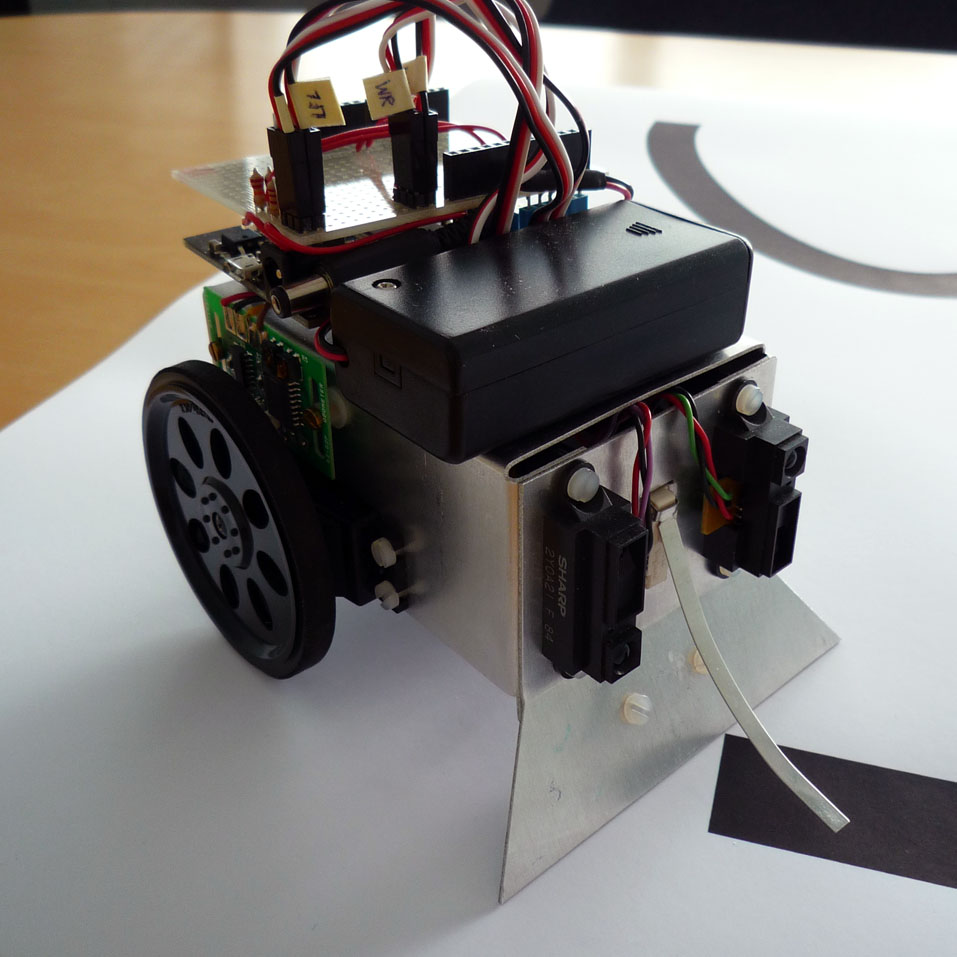
\includegraphics[width=0.3\linewidth]{linefollower/r2g2p_netduino}
      \label{fig:linefollower_sm}
}
\subfigure[A line-follow path]
{
      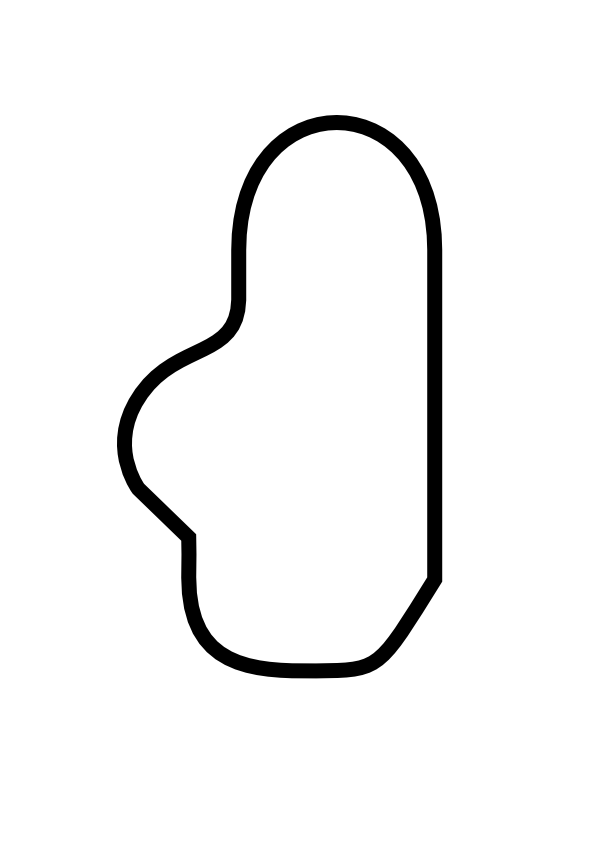
\includegraphics[width=0.3\linewidth]{linefollower/map}
      \label{fig:linefollower_3dpath}
}
\subfigure[3D representation of the line-following robot]
{
      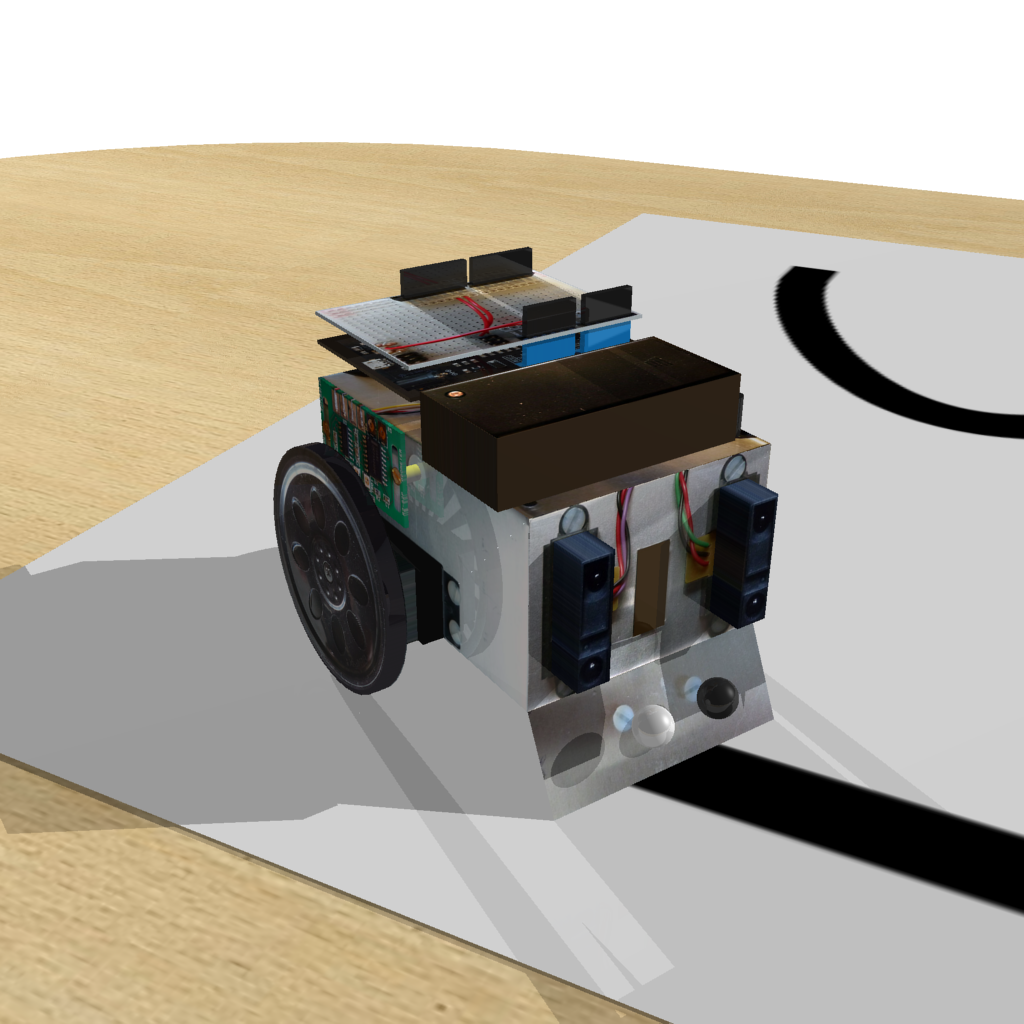
\includegraphics[width=0.3\linewidth]{linefollower/robot_inside}
      \label{fig:linefollower_3d}
}
\caption{The line-following robot}
\label{fig:linefollowoverview}
\end{center}
\end{figure}

\subsection{Usage}
\label{sec:linefollower_usage}

The example is available from the INTO-CPS application menu at \emph{File>Import Example Project} or at  \url{https://github.com/INTO-CPS-Association/example-line_follower_robot} in the \emph{master} branch. There are several subfolders for the various elements: DSEs - contains various work in progress DSE scripts to alter CT and DE parameters; \texttt{FMU} -- contains the various FMUs of the study; \texttt{Models} -- contains the constituent models defined using the INTO-CPS simulation technologies; \texttt{Multi-models} -- contains the multi-model definitions and co-simulation configurations -- with 3D and non-3D options, and also with and without the use of replicated FMUs; \texttt{SysML} -- contains the SysML models defined for the study; \texttt{resources} -- various images for the purposes of the readme file; and \texttt{userMetricScripts} -- contains files for DSE analysis. 

The \texttt{case-study\_line\_follower\_robot} folder can be opened in the INTO-CPS application to run the various co-simulations as detailed in this document. To run a simulation, expand one of the multi-models and click `Simulate' for an experiment. 


%\subsection{INTO-CPS Technology}
%
%We demonstrate the use of the INTO-CPS SysML profile in Section~\ref{sec:linefollwerrobot_into_sysml}. Based upon the design architecture defined using the SysML profile, a multi-model is constructed in Section~\ref{sec:linefollwerrobot_into_mm} along with the defined connections.

\subsection{INTO SysML profile}
\label{sec:linefollwerrobot_into_sysml}

\subsubsection*{Non replicated sensors}
The multi-model architecture, defined in the INTO-CPS SysML profile, shows that the \emph{Robot} system is comprised of up to 5 components, as shown in the Architecture Structure Diagram in Figure~\ref{fig:linefollowasd}. This comprises the following components: \emph{Body}, \emph{Sensor1} and \emph{Sensor2} physical components, a \emph{Controller} cyber component and a \emph{3DVisualisation} visualisation component.

\begin{figure}[htb!]
\begin{center}
     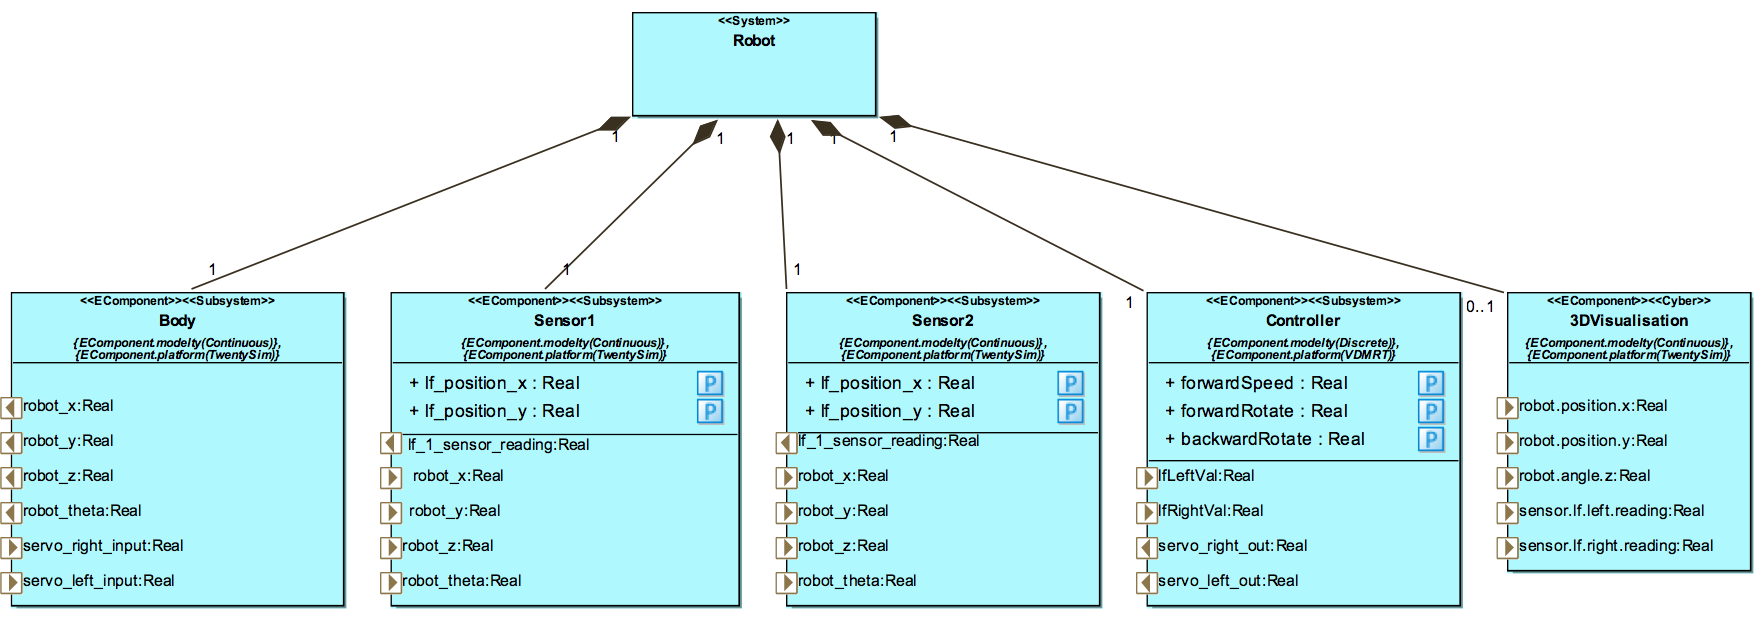
\includegraphics[width=1\linewidth]{linefollower/r2g2p_asd.png} 
\caption{The line-following robot Architecture Structure Diagram}
\label{fig:linefollowasd}
\end{center}
\end{figure}


Two Connection Diagrams are defined. The first, in Figure~\ref{fig:linefollowcd1}, shows connections only between the \emph{Controller}, \emph{Body}, \emph{Sensor1} and \emph{Sensor2} component instances. Broadly speaking: the \emph{Controller} receives sensor readings from both \emph{Sensor1} and \emph{Sensor2} components; the \emph{Controller} in turn sends servo commands to the \emph{Body} component; and finally the \emph{Body} sends the robot position to both sensor components. 

\begin{figure}[htb!]
\begin{center}
     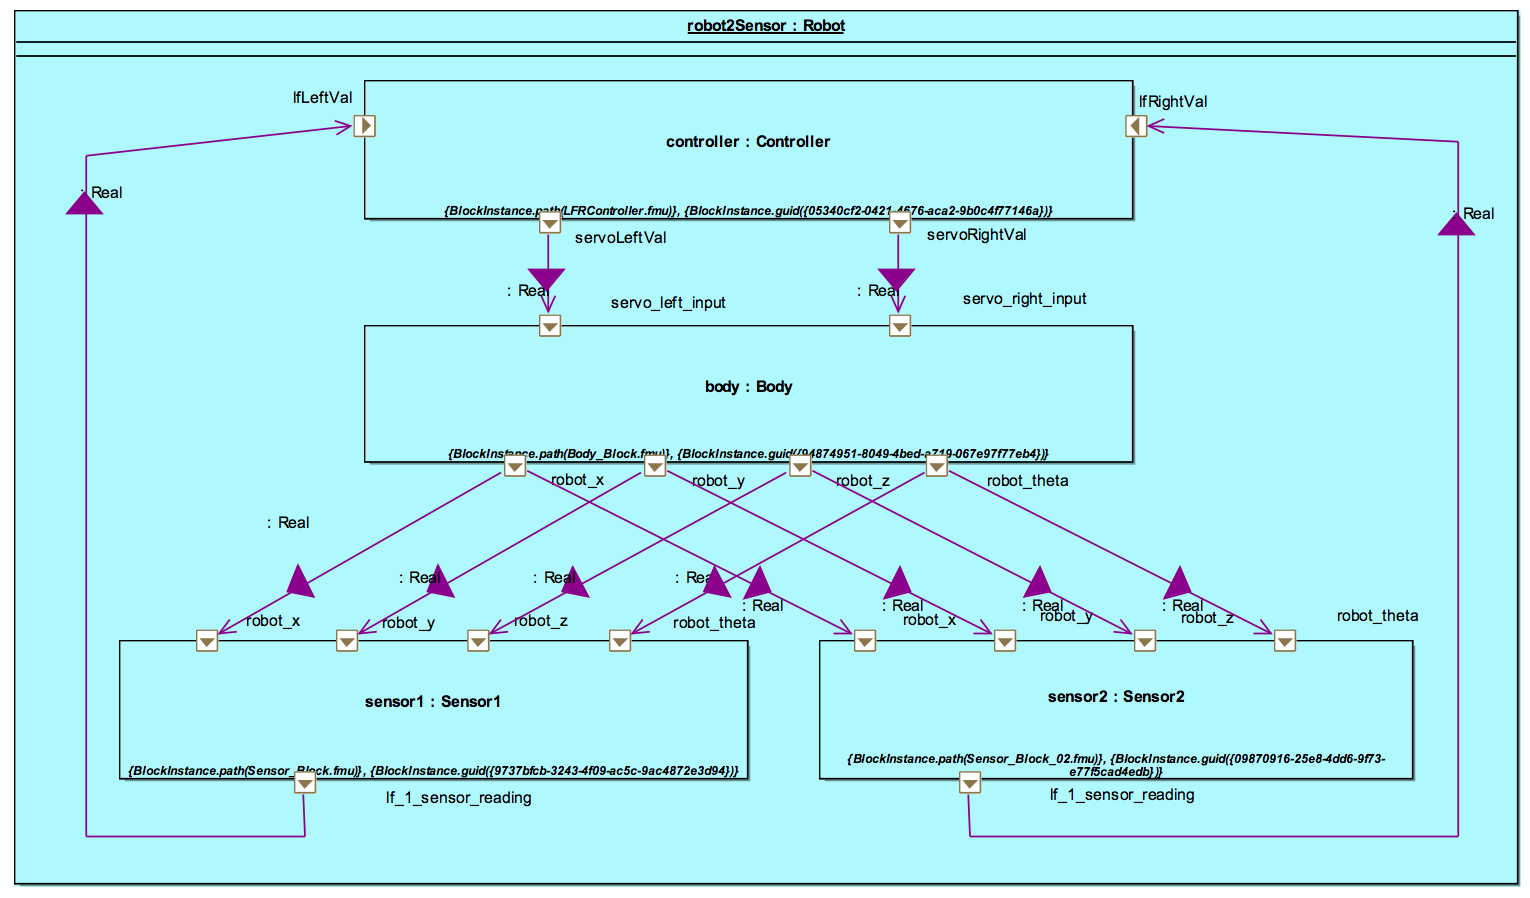
\includegraphics[width=0.9\linewidth]{linefollower/r2g2p_cd_non3d.png} 
\caption{The line-following robot Connections Diagram}
\label{fig:linefollowcd1}
\end{center}
\end{figure}

Figure~\ref{fig:linefollowcd2} shows the alternative CD in which the \emph{3DVisualisation} component is used. In this diagram, the \emph{3DVisualisation} component receives data from the \emph{Body} on the robot position, and the sensor readings from the two sensors. Unlike other examples using the visualisation component type, no additional internal data is required to be exposed by the existing components. 

\begin{figure}[htb!]
\begin{center}
     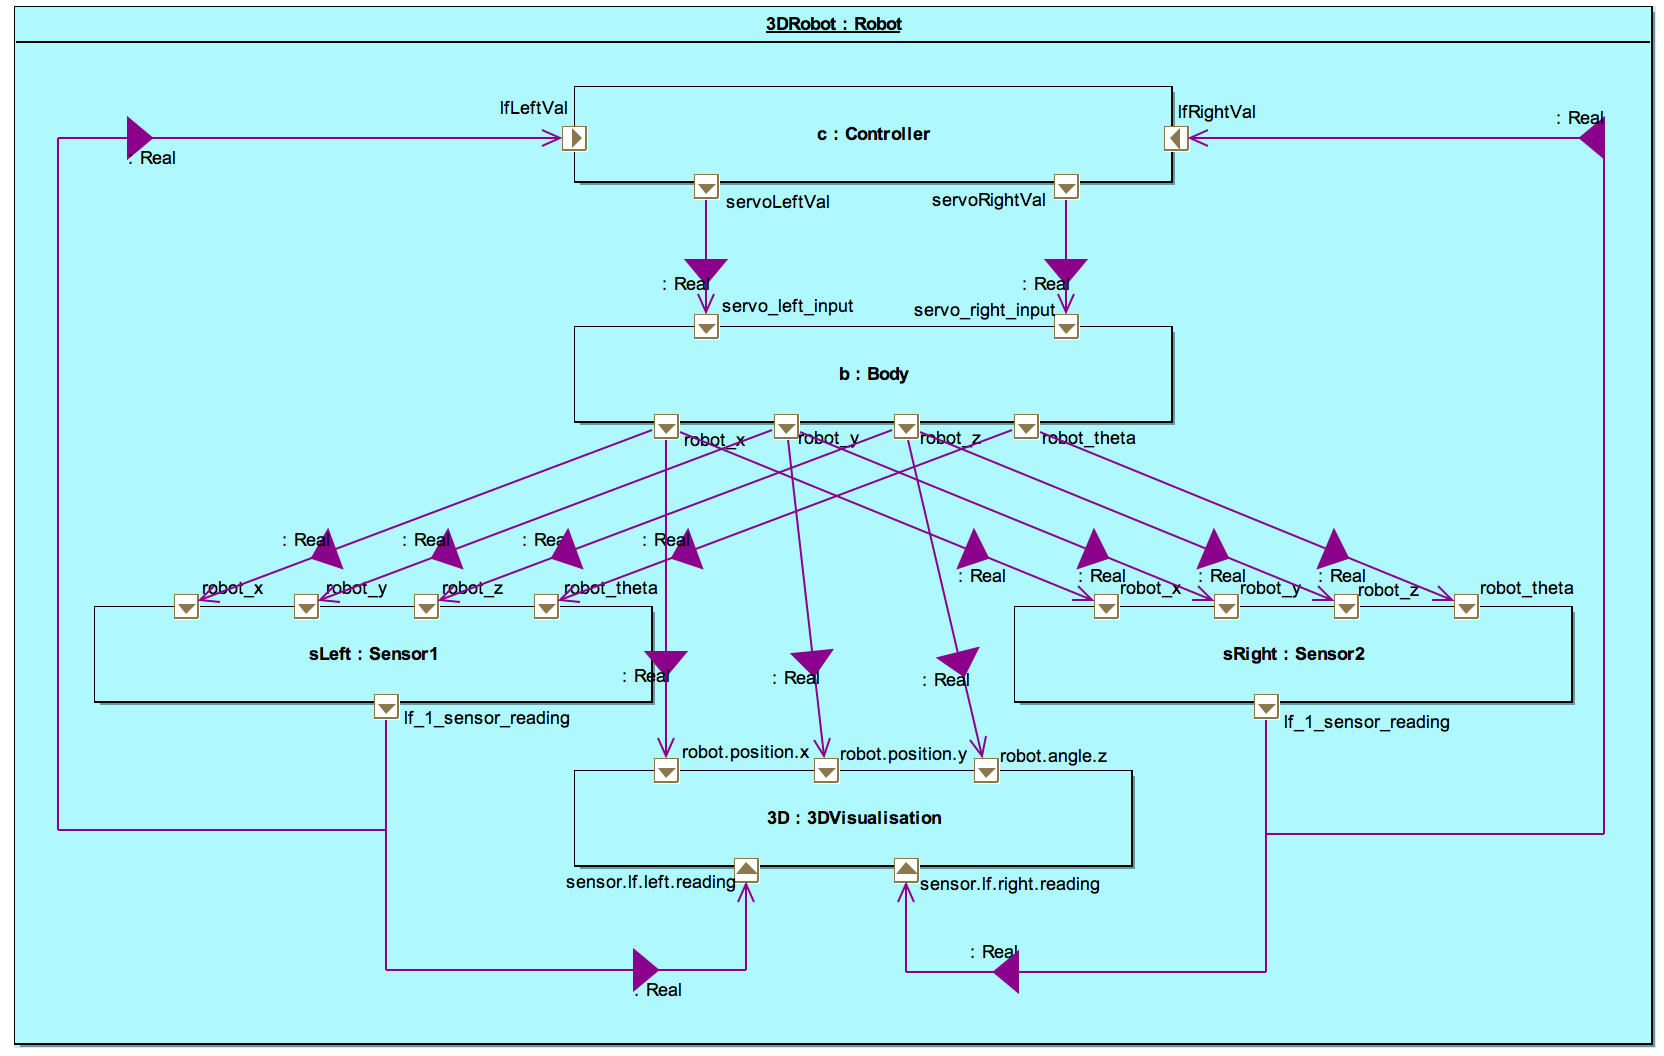
\includegraphics[width=0.9\linewidth]{linefollower/r2g2p_cd_nonrep_3d.png} 
\caption{The line-following robot Connections Diagram}
\label{fig:linefollowcd2}
\end{center}
\end{figure}

\subsubsection*{Replicated sensors}

An alternative architecture has also been defined in which we use replication offered by 20-sim and OpenModelica FMUs. The ASD in Figure~\ref{fig:linefollowasdrep} demonstrates the use of two instances of the same \emph{Sensor} component type.

\begin{figure}[htb!]
\begin{center}
     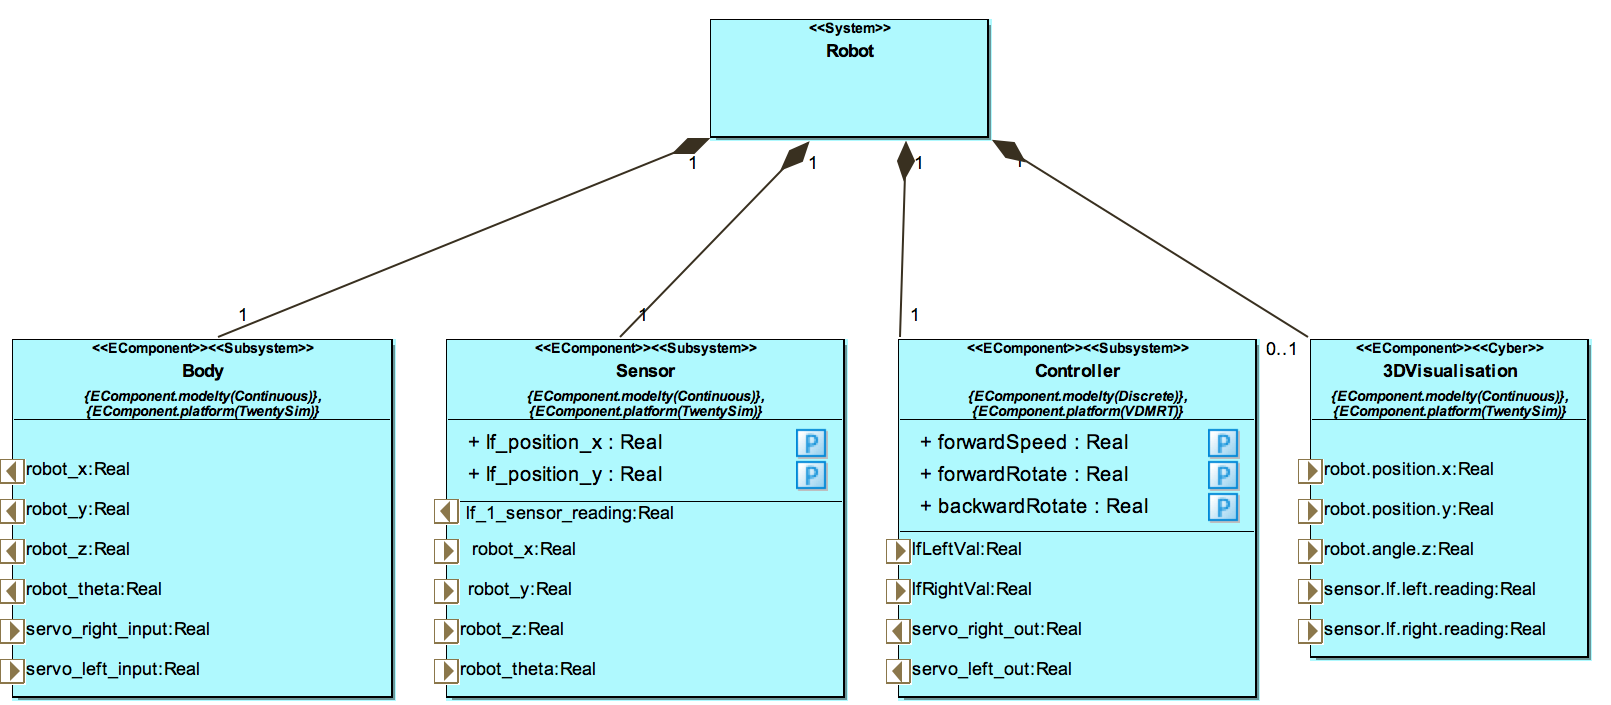
\includegraphics[width=0.8\linewidth]{linefollower/r2g2p_asd_rep.png} 
\caption{The line-following robot Architecture Structure Diagram with replicated sensors}
\label{fig:linefollowasdrep}
\end{center}
\end{figure}

The CDs for this SysML model are similar to the non-replicated sensor model. The only difference is the change of sensor types for the two sensor instances -- this is shown in Figures~\ref{fig:linefollowcdrep1} and~\ref{fig:linefollowcdrep2}.

\begin{figure}[htb!]
\begin{center}
     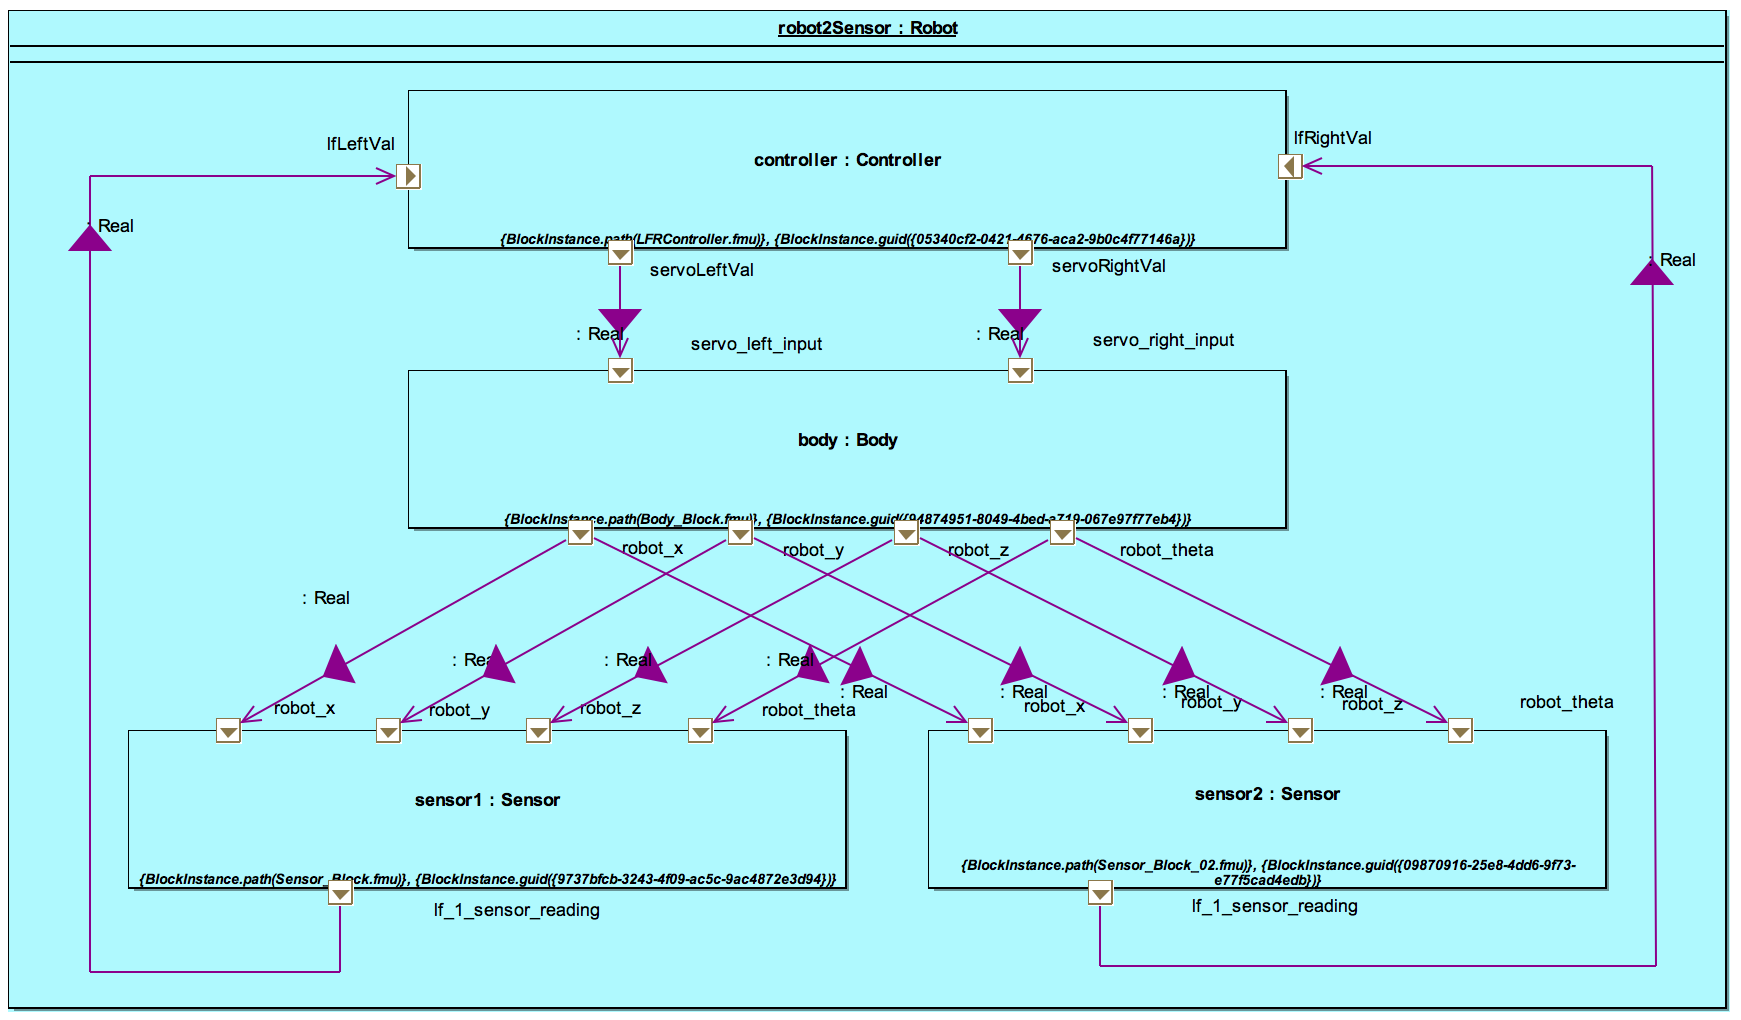
\includegraphics[width=0.9\linewidth]{linefollower/r2g2p_cd} 
\caption{The line-following robot Connections Diagram}
\label{fig:linefollowcdrep1}
\end{center}
\end{figure}

\begin{figure}[htb!]
\begin{center}
     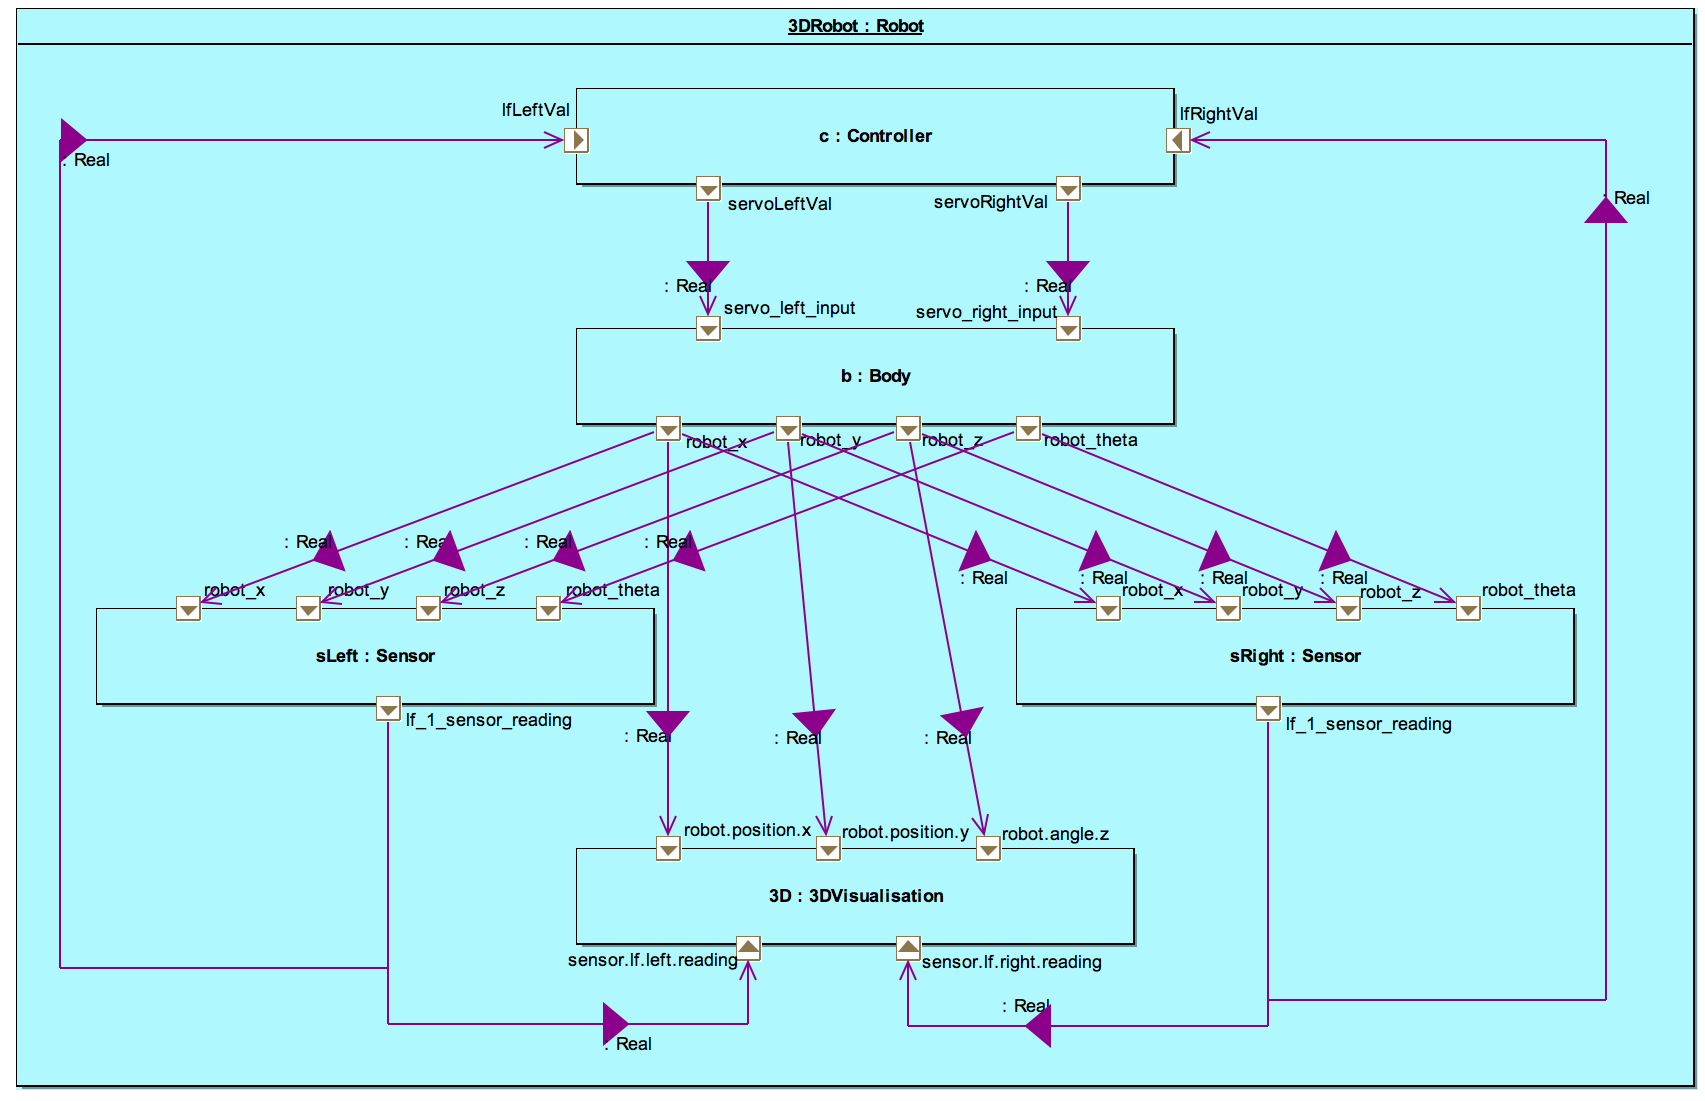
\includegraphics[width=0.9\linewidth]{linefollower/r2g2p_cd_rep_3d} 
\caption{The line-following robot Connections Diagram}
\label{fig:linefollowcdrep2}
\end{center}
\end{figure}


\subsection{Multi-model}
\label{sec:linefollwerrobot_into_mm}

\subsubsection{Models}
%The multi-model produced and analysed using INTO-CPS technology stems from the baseline Crescendo co-model. The multi-model comprises 3 models, splitting the Crescendo model as depicted in Figure~\ref{fig:linefollowsplit}.  This example, therefore is a multi-CT model, with a single DE model. 
%
%\begin{figure}[htb!]
%\begin{center}
%     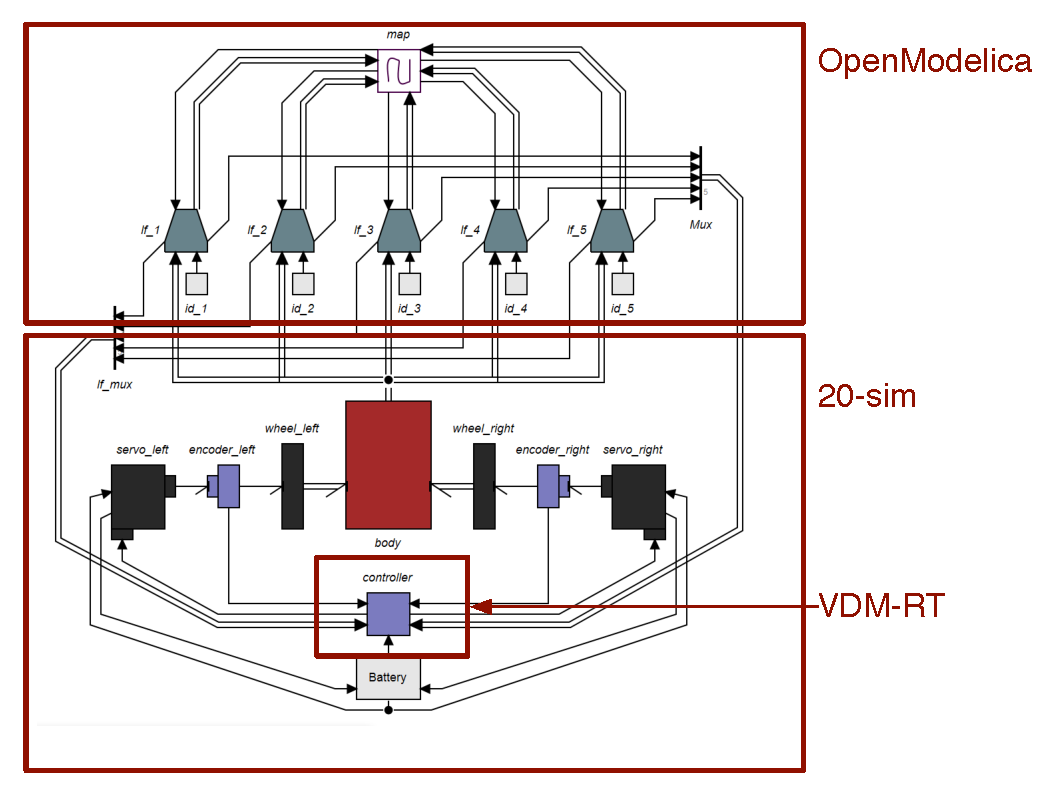
\includegraphics[width=0.65\linewidth]{linefollower/r2g2p_ct_split} 
%\caption{Splitting the line-following robot Crescendo model}
%\label{fig:linefollowsplit}
%\end{center}
%\end{figure}

Based upon the two SysML models, we define four different simulation models: a 20-sim \emph{Body} model; a VDM-RT \emph{Controller} model; a 20-sim \emph{Sensor} models; and one OpenModellica \emph{Sensor} model.  

\begin{description}
\item[Body] To define the 20-sim Body subsystem, Figure~\ref{fig:linefollow20simmod}, we first define a top-level decomposition with a \emph{Body\_Block} and a block to represent the body's \emph{Environment}. 

\begin{figure}[htb!]
\begin{center}
  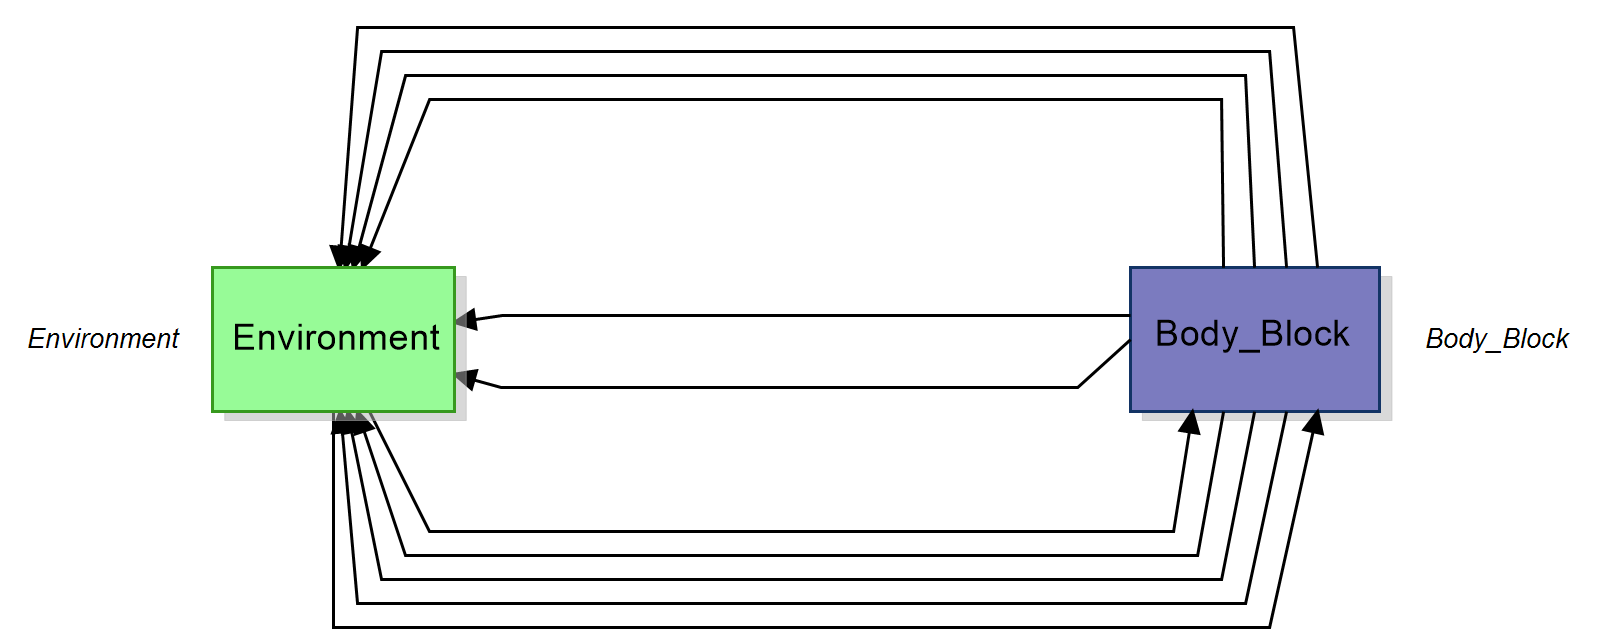
\includegraphics[width=0.65\linewidth]{linefollower/r2g2t_mod2} 
\caption{Top-level 20-sim model of the line-following robot \emph{Body}}
\label{fig:linefollow20simmod}
\end{center}
\end{figure}

Decomposing the \emph{Body\_Block} further, the 20-sim model is defined as in Figure~\ref{fig:linefollowbody20simmm}. Blocks are defined for servos, encoders, wheels, the battery and the body itself. A collection of input and output ports are defined: ports to output the robot position (\emph{robot\_x}, \emph{robot\_y}, \emph{robot\_z} and \emph{robot\_theta}); ports to output wheel rotation values (\emph{wheel\_left\_rotation} and \emph{wheel\_right\_rotation}); a port to output the battery usage (\emph{total\_energy\_used}); and ports for inputting servo power values (\emph{servo\_left\_input} and \emph{servo\_right\_input}).

\begin{figure}[htb!]
\begin{center}
     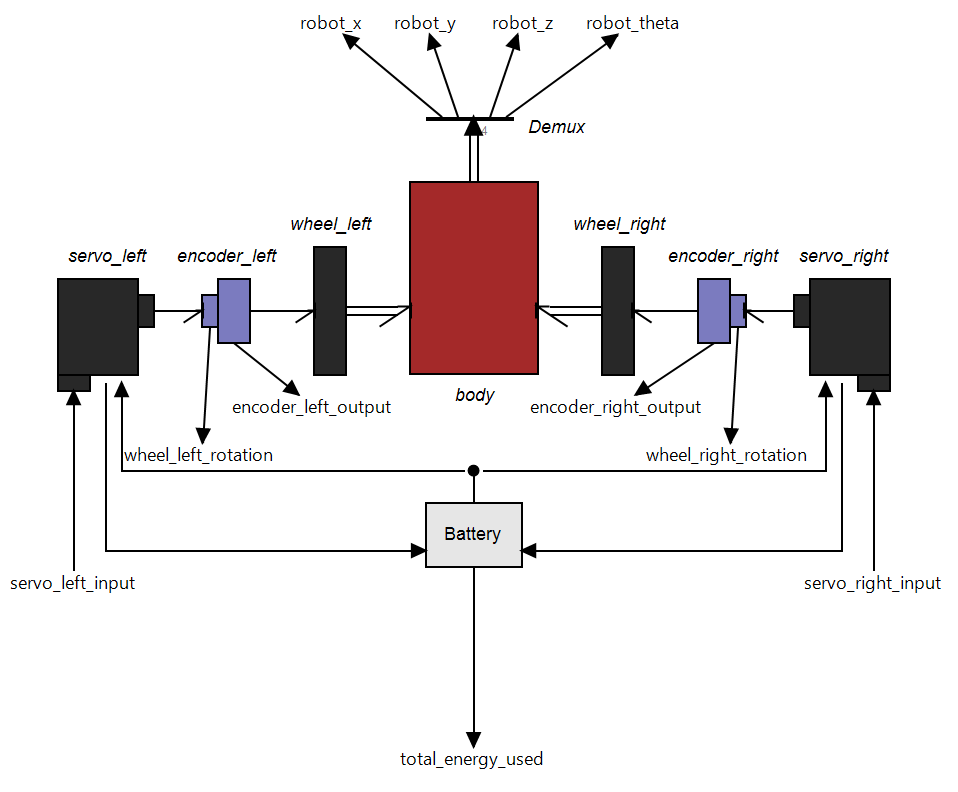
\includegraphics[width=0.7\linewidth]{linefollower/r2g2p_body} 
\caption{20-sim model of the line-following robot \emph{Body}}
\label{fig:linefollowbody20simmm}
\end{center}
\end{figure}



\item[20-sim\_Sensor] The \emph{Sensor\_Block} is shown in Figure~\ref{fig:linefollow20simsensor}.  For the non-replicated version, we change the names of the \emph{Sensor\_Block} to generate different FMUs.

\begin{figure}[htb!]
\begin{center}
 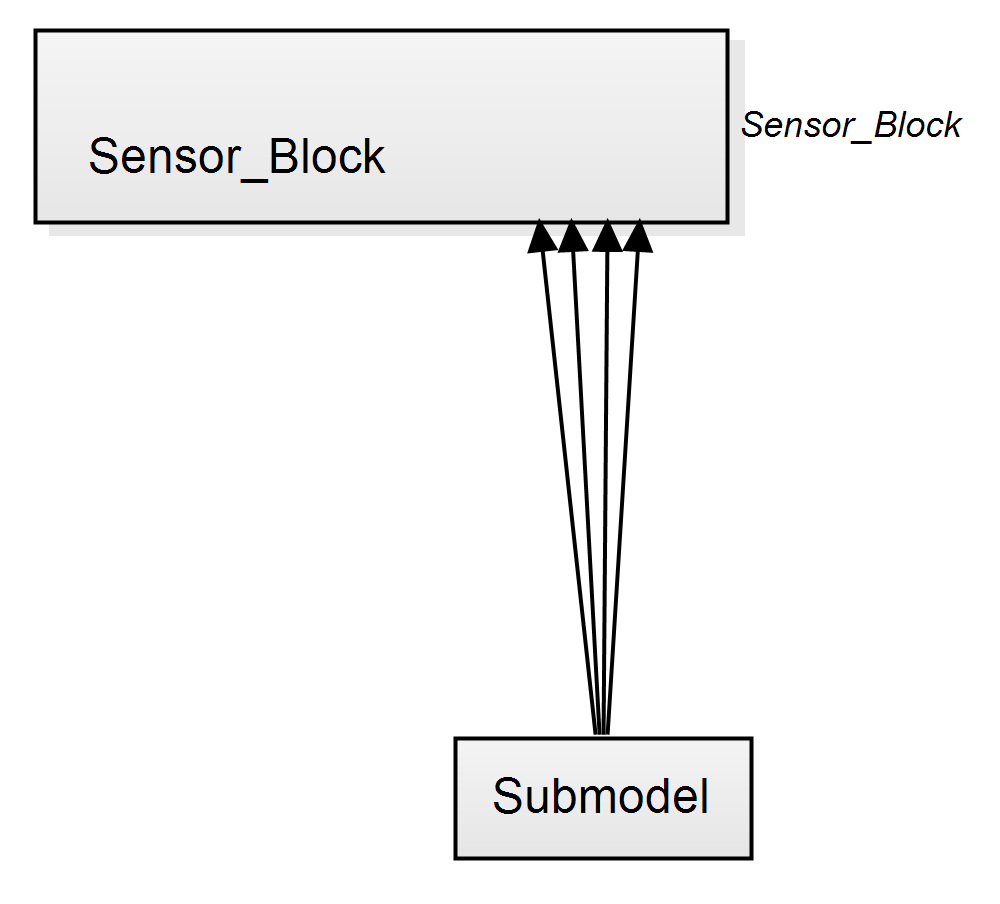
\includegraphics[width=0.45\linewidth]{linefollower/r2g2p_sensor1} 
\caption{Top-level 20-sim model of the line-following robot \emph{Sensor}}
\label{fig:linefollow20simsensor}
\end{center}
\end{figure}

Decomposing the \emph{Sensor\_Block}, we see the internal elements of the sensor -- shown in Figure~\ref{fig:linefollowbody20sensor2}. The sensor receives the robot position from its environment, calculating its position in the world using the \emph{line\_follow\_x} and \emph{line\_follow\_y} design parameters. This position information is passed to the \emph{map} block, which takes a sample of values and passes a raw reading back to the sensors. The sensors then convert this to an 8-bit value, taking into account realistic behaviours: ambient light levels, a delayed response to changes, and A/D conversion noise. The final sensor reading is output on the \emph{lf\_1\_sensor\_reading} port. 

\begin{figure}[htb!]
\begin{center}
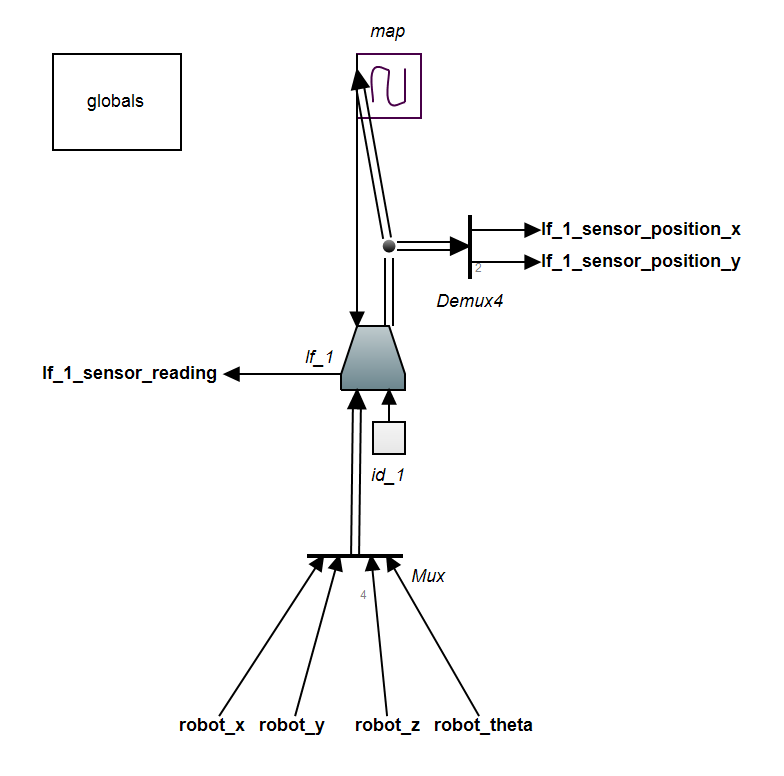
\includegraphics[width=0.5\linewidth]{linefollower/r2g2p_sensor2} 
\caption{20-sim model of the line-following robot \emph{Sensor}}
\label{fig:linefollowbody20sensor2}
\end{center}
\end{figure}

\item[OM\_Sensor] The OpenModelica version of the sensor is provided in the \emph{LineFollower} package. The 
\emph{SensorBlock1.mo} element, shown in Figure~\ref{fig:linefollowbodyOMsensor} corresponds to the 20-sim model shown in Figure~\ref{fig:linefollowbody20sensor2}. The model has the same interface, with internal elements for reflectivity, ambient light, and A/D conversion noise.

\begin{figure}[htb!]
\begin{center}
\subfigure[Top-level view]
{
      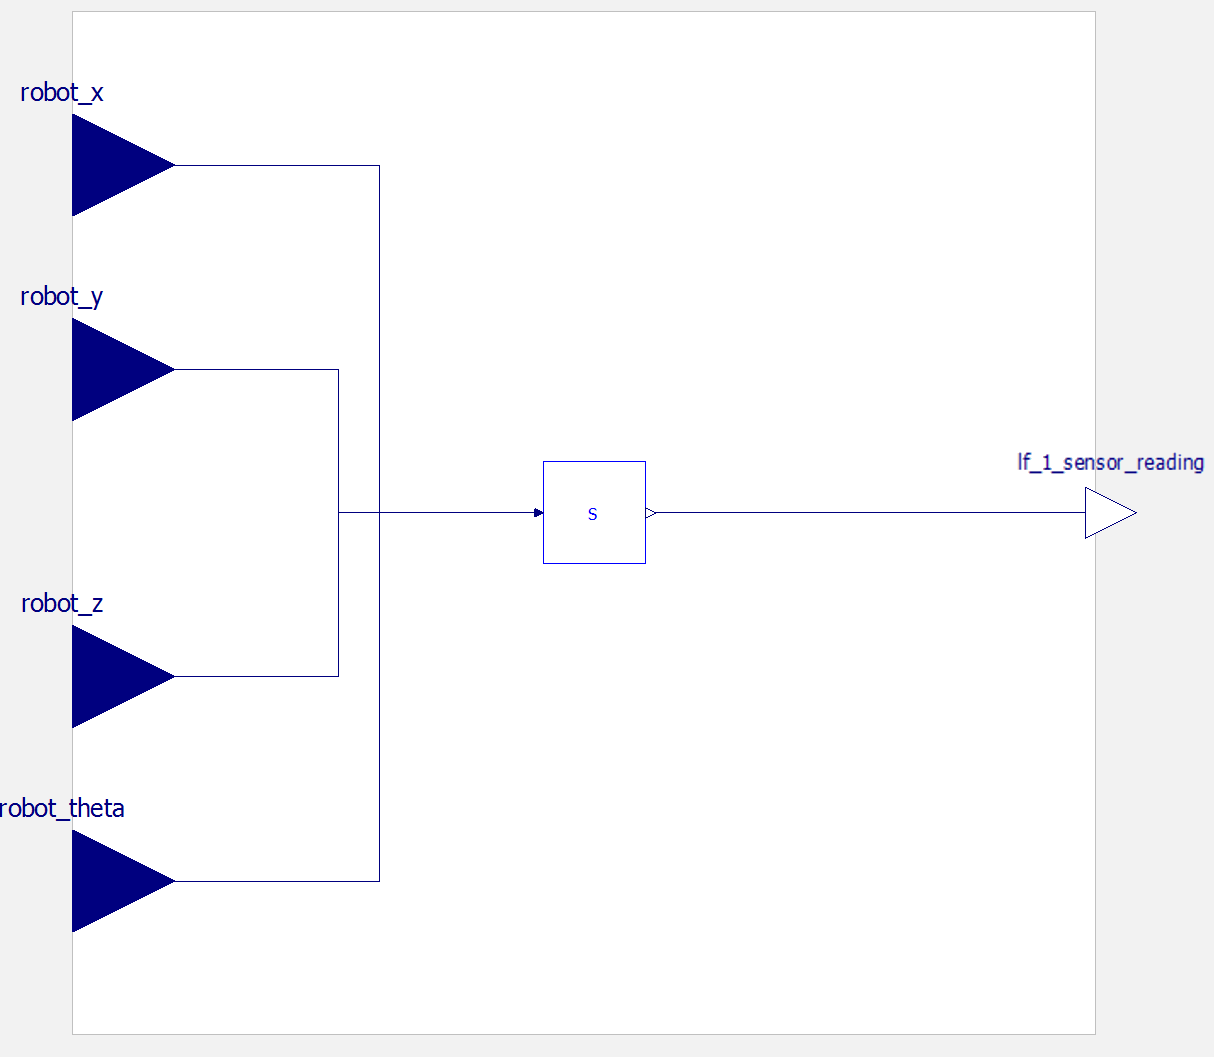
\includegraphics[width=0.45\linewidth]{linefollower/r2g2p_sensor_om_2}
      \label{fig:linefollower_om_s1}
}
\subfigure[Low-level view]
{
      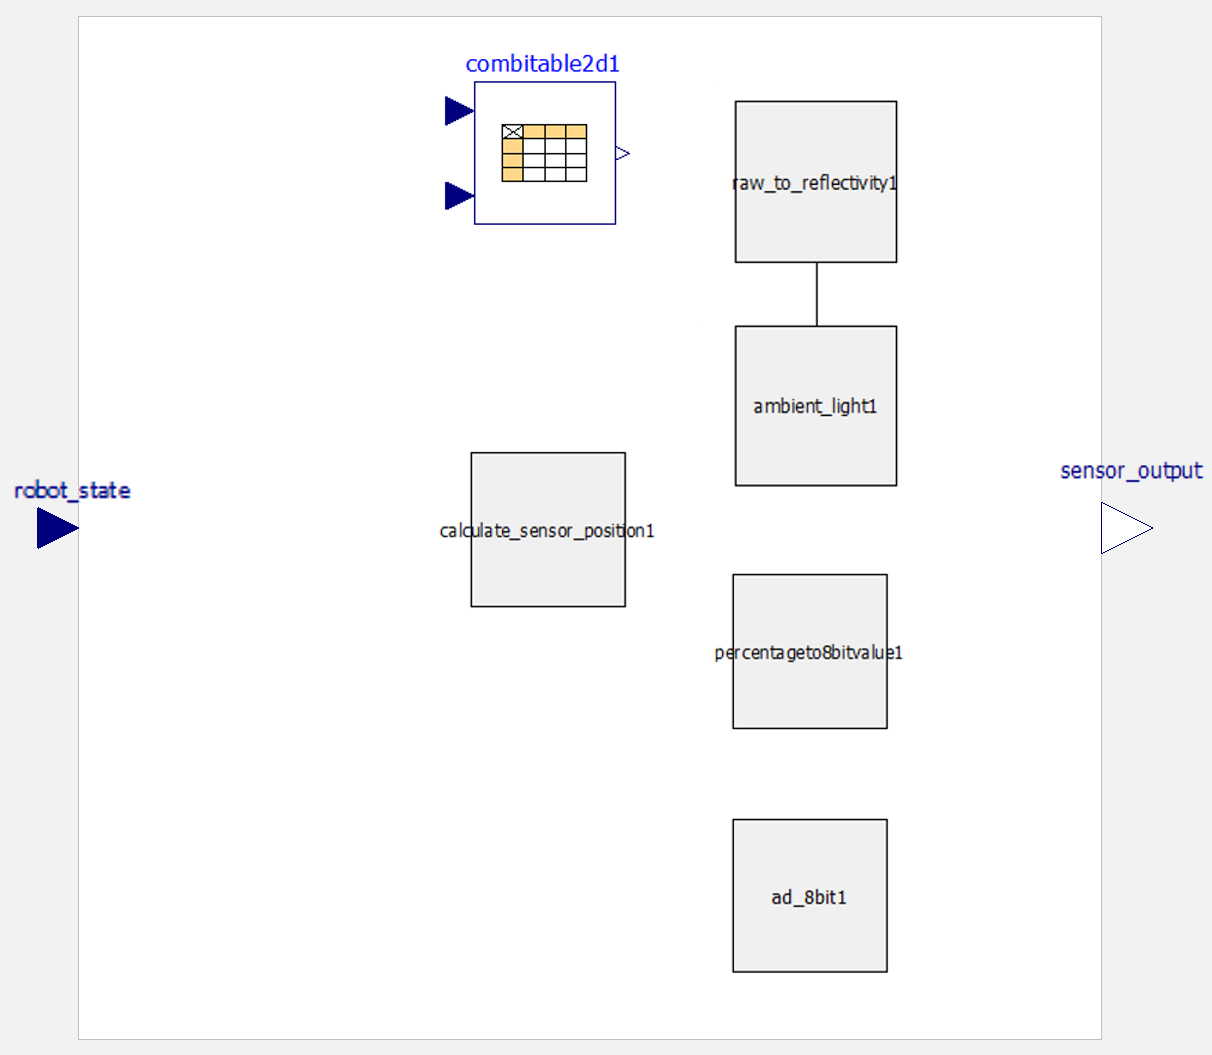
\includegraphics[width=0.45\linewidth]{linefollower/r2g2p_sensor_om}
      \label{fig:linefollower_om_s2}
}
\caption{OpenModelica model of the line-following robot \emph{Sensor}}
\label{fig:linefollowbodyOMsensor}
\end{center}
\end{figure}



\item[Controller] The VDM-RT controller model is conceptually unchanged from the original Crescendo controller. The architecture of this model is in Figure~\ref{fig:linefollowbodyvdm}. The \emph{Controller} model comprises a \emph{System} class which contains a \emph{HardwareInterface} instance which contains references to the inputs, outputs and design parameters. The \emph{System} class also contains a \emph{Controller} class which makes the control decisions. The decisions are based upon sensor readings obtained from two instances of the \emph{RobotSensor} class, and decisions are sent to the two \emph{RobotServo} instances. In this model, a simple algorithm is used: when both sensors see a black line the robot moves forward (both servos are set to the same value), when only the right sensor sees the black line the robot moves left -- and vice-versa.


\begin{figure}[htb!]
\begin{center}
     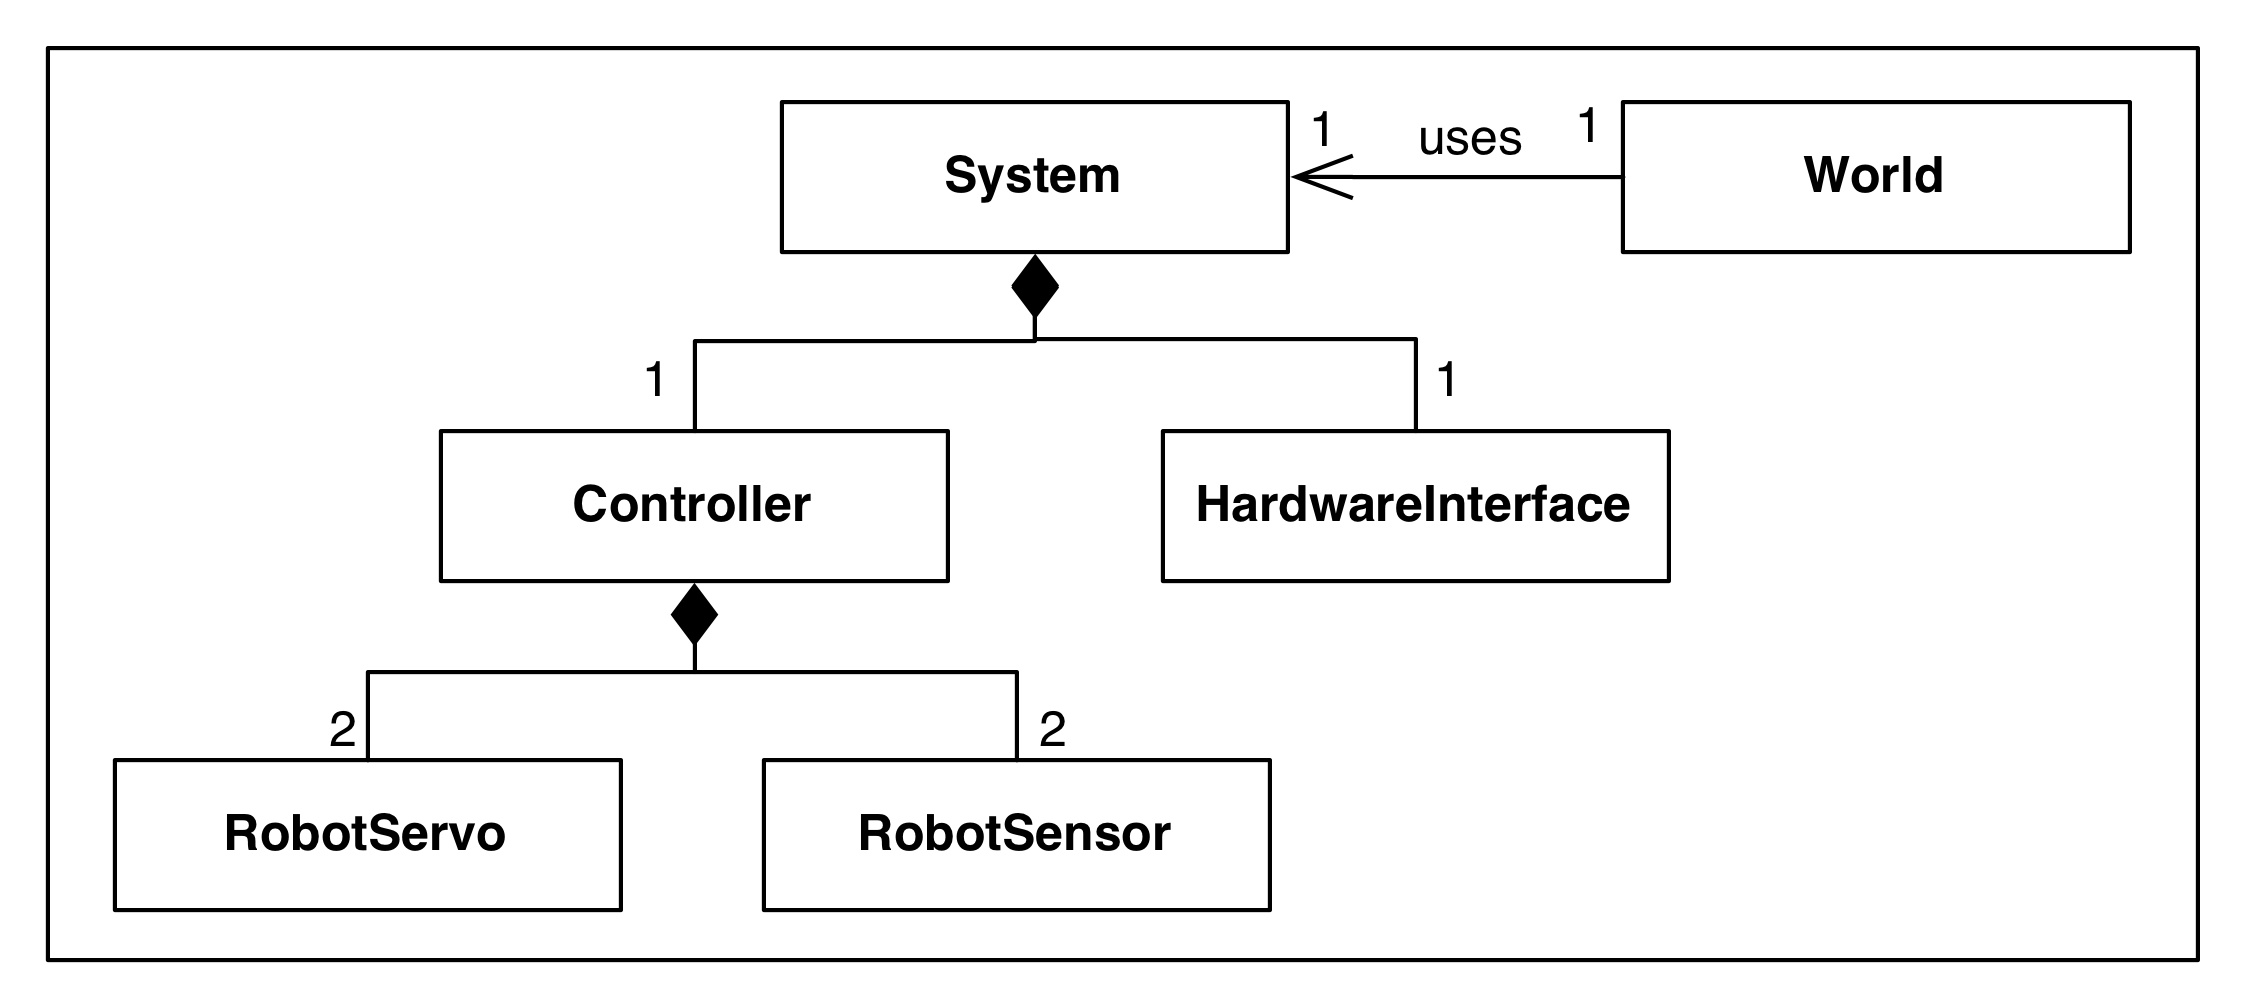
\includegraphics[width=0.8\linewidth]{linefollower/r2g2p_vdm} 
\caption{UML representation of line-following robot \emph{Controller} model}
\label{fig:linefollowbodyvdm}
\end{center}
\end{figure}

\end{description}

\subsubsection{Configuration}

There are several connections between the models in the multi-model.

The first collection of connections is between the Body 20-sim model and the Controller VDM-RT model. In this collection, there are two connections corresponding to signals for the actuators that power the motors for the wheels:
\begin{itemize}
  \item from the \emph{Controller} \texttt{servoLeftVal} variable of type real to the \texttt{servo\_left\_input} port of the \emph{Body}; and
  \item from the \emph{Controller} \texttt{servoRightVal} variable of type real to the \texttt{servo\_right\_input} port of the \emph{Body}. 
\end{itemize} 

The second collection of connections is between the Sensor models and the Controller VDM-RT model. For each sensor there is one connection to the controller to represent inputs from line-following sensors that can detect areas of light and dark on the ground. Therefore for a two-sensor model there are two connections:
 \begin{itemize}
  \item from the \emph{Sensor1}\footnote{Sensor1 is an instance of either the non-replicated \emph{Sensor\_Block1} or the replicated \emph{Sensor\_Block}} \texttt{lf\_1\_sensor\_reading} port to the \emph{Controller} \texttt{lfLeftVal} variable; and 
  \item from the \emph{Sensor2}\footnote{Sensor2 is an instance of either the non-replicated \emph{Sensor\_Block2} or the replicated \emph{Sensor\_Block}} \texttt{lf\_1\_sensor\_reading} port to the \emph{Controller} \texttt{lfRightVal} variable. 
\end{itemize}

  
A third collection of connections exist between the body and the sensors related to the robot position:
 \begin{itemize}
  \item from the \emph{Body} \texttt{robot\_x} port to the \emph{Sensor} \texttt{robot\_x} port; 
  \item from the \emph{Body} \texttt{robot\_y} port to the \emph{Sensor} \texttt{robot\_y} port; 
  \item from the \emph{Body} \texttt{robot\_z} port to the \emph{Sensor} \texttt{robot\_z} port; and 
  \item from the \emph{Body} \texttt{robot\_theta} port to the \emph{Sensor} \texttt{robot\_theta} port. 
\end{itemize}
  
A collection of multi-models   is provided in the study for combinations of 20-sim and OpenModelica models.
  
Several shared design parameters are present also: the separation of the line-following sensors from the centre line, in metres (\emph{line\_follow\_x}); and the distance forward of the line-following sensors from the centre of the robot, in metres (\emph{line\_follow\_y}). In addition, design parameters are set for the controller: the \emph{forwardSpeed} and values for rotation -- \emph{forwardRotate} and \emph{backwardRotate}.
  

\subsection{Co-simulation}
\label{sec:fcu_into_co}

For all these multi-models, co-simulations require approximately 25-30 seconds of simulation to traverse the full map, using a fixed step size of 0.01 seconds. The example has co-simulation set ups for each multi-model and the non-3D models have live stream enabled for the sensed values from sensor1 and sensor2.

\subsection{Analyses and Experiments}
\label{sec:fcu_analyses}

Below we detail some useful experiments to demonstrate features of the INTO-CPS tool chain.

\subsubsection{Change FMUs/parameters}

The case study has several Sensor FMUs. In the multi-model configuration it is possible to swap the FMU allocated to each sensor instance of the multi-model. We can therefore compare the results of co-simulation using a combination of 20-sim sensors (the replicated \emph{Sensor\_Block.fmu}, or \emph{Sensor\_Block1.fmu} and \emph{Sensor\_Block2.fmu}) and OpenModelica sensors (replicated, or some combination of \emph{LineFollower\_Examples\_SensorBlock1.fmu} and \emph{LineFollower\_Examples\_SensorBlock2.fmu}). 

In addition, there are parameters defined for the two sensors (an x and y position \texttt{lf\_position\_x} and \texttt{lf\_position\_y}), and of the controller (forward and rotational speeds \emph{forwardSpeed}, \emph{forwardRotate} and \emph{backwardRotate}). Experiments may be carried out by defining different values for these to model different placement of the sensors on the robot and altering the robot speeds,. 

\subsubsection{Simulations due to previous results}

Simulations can be replayed using different design parameter values to change the position of the robot sensors. Changing these parameters amounts to changing the design of the robot - some value pairs will produce robots which perform in some way better (e.g. have a faster lap time) and others will result in robots which cannot follow the line.

\subsubsection{Design Space Exploration}

Several Design Space Exploration experiments have been included in this pilot. They are described in more detail in Deliverable D5.3e~\cite{INTOCPSD5.3e}, and we give an overview of the different experiments here. 

\begin{description}
   \item[lfr-2sensorPositions:] This experiment uses four design parameters, but only varies one. The \texttt{lf\_position\_y} of \emph{sensor1} may be either $0.07$ or $0.13$. Four objective scripts are used: \emph{meanSpeed}, \emph{lapTime}, \emph{maxCrossTrackError} and \emph{meanCrossTrackError}. The Pareto ranking only uses the \emph{lapTime} and \emph{meanCrossTrackError} objectives; these determine the time taken for the robot to perform one lap of the map, and also the mean error the robot makes when following the line. 
   
   \item[lfr-8controllerValues:] This experiment uses and varies three parameters. These parameters are all on the cyber-side of the multi-model -- effecting the robot speeds set by the controller. For each (\texttt{forwardSpeed}, \texttt{forwardRotate} and \texttt{backwardRotate}), two possible values are defined - giving a design space of 8 designs. The same four objective scripts are used as above with the same Pareto ranking.
   
   \item[lfr-16sensorPositionsConstrained:] This experiment is a more complex version of the \textbf{lfr-2sensorPositions} experiment in that it varies all four design parameters -- the \texttt{lf\_position\_x} and \texttt{lf\_position\_y} coordinates of both \emph{sensor1} and \emph{sensor2}. Two possible values are defined for each parameter -- giving a 16-design space. A constraint is defined for the parameters, which limits this design space to include only those designs which have the same y coordinate and the same absolute x coordinate. The same four objective scripts are used as above with the same Pareto ranking.
   
   \item[lfr-216controllerValues:] This expands the \textbf{lfr-8controllerValues} experiment, providing 6 speed values for the Controller parameters (\texttt{forwardSpeed}, \texttt{forwardRotate} and \texttt{backwardRotate}), producing a design space of 216 designs. The same four objective scripts are used as above with the same Pareto ranking.
   
   \item[lfr-2187ControllerAndSensors:] The final experiment combines DSE on both DE and CT models. Providing an insight into the possibility to trade-off between development effort on the cyber or physical side. In this experiment there are 3 possible positions for each of the the \texttt{lf\_position\_x} and \texttt{lf\_position\_y} coordinates of both \emph{sensor1} and \emph{sensor2}, and also 3 values for the  Controller parameters (\texttt{forwardSpeed}, \texttt{forwardRotate} and \texttt{backwardRotate}). This produces a design space of 2187 designs. The same four objective scripts are used as above with the same Pareto ranking.
   
\end{description}

\subsubsection{Test Automation and Model Checking}
\label{sec:lfr_ta}
\graphicspath{ {linefollower/TA/} }

In this pilot study, we apply test automation only to the controller, instead of the system in the FCU study. The continuous body and sensors are rather complex in order to be modelled in a test model in SysML in Modelio by state machine diagrams. Therefore, only the discrete part \emph{Controller} will be tested. In addition, the \emph{Controller} is a simplified version which is similar to the VDM model in \emph{LFRController.fmu}. In this model, the parameters $forwardSpeed$, $forwardRotate$ and $backwardRotate$ are fixed to 4.0, 5.0 and 1.0 respectively. We implement a SUT manually in C. Then model checking is applied to check a couple of properties of the test model, and finally test automation to test whether the SUT is a correct implementation of the test model.

\paragraph{Test Model}
The overall architecture and connection diagrams of this test model are omitted for brevity. The \emph{SystemUnderTest} includes only one block \emph{LFR\_CTRL}. 
\subparagraph{Inputs and Outputs}
The \emph{SystemUnderTest} receives the following inputs (stimuli) from the \emph{TestEnvironment}:
\begin{itemize}
    \item $sensorLeftVal$ %: the reading of the left sensor; 
    \item $sensorRightVal$ %: the reading of the right sensor.
\end{itemize}

The \emph{SystemUnderTest} provides the following observable outputs to the \emph{TestEnvironment}:
\begin{itemize}
    \item $servoLeft$ %: the signal to the left actuator (to drive the left wheel);
    \item $servoRight$ %: the signal to the right actuator (to drive the right wheel).
\end{itemize}

\subparagraph{Constant Variables and Local Variables}
Preliminarily, we intend to define three constant variables $forwardSpeed$, $forwardRotate$ and $backwardRotate$ of which the access model property is set as \T{Read}. Then in the state machine diagram of \emph{LFR\_CTRL}, we use these variables to refer to constants. However, these constant variables are not supported in RT-Tester. Their initial values are all set to 0 when parsing the test model. Alternatively, we can initialise them to constants in the first state just after the \T{Init} state, or just use hard-coded constants in the test model (the way used in this study).

Another two local variables $preServoLeft$ and $preServoRight$ are declared to store previously output values of $servoLeft$ and $servoRight$ separately. And their access model property is set to \T{Read/Write}.

\subparagraph{State Machine Diagram}
The state machine diagram of \emph{FCU\_CTRL} is given in Figure~\ref{fig:lfr-sm-diagram}. It is worth noting that
\begin{itemize}
    \item This model is based on a very basic variation of the controller and it only provides four possible outputs.
    \item The texts in blue actually are not a part of the model and they are annotations only to illustrate associated expression for each guarded transition (because the expressions cannot be seen from the diagram directly).
    \item When both $sensorLeftVal$ and $sensorRightVal$ are larger than or equal to $150$, our model outputs the previously stored $preServoLeft$ and $preServoRight$. It means the outputs have not changed. 
\end{itemize}
\begin{figure}[htb!]
    \centering
  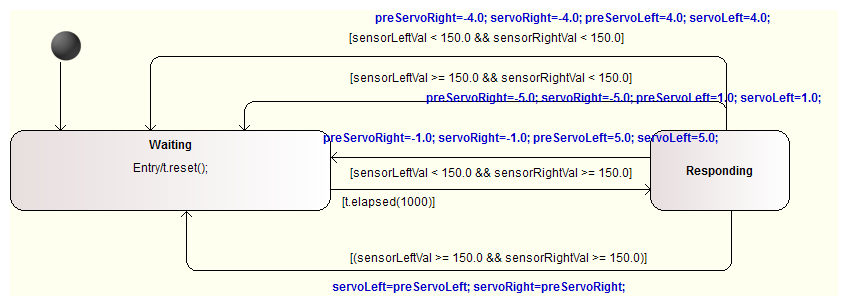
\includegraphics[width=1.0\textwidth]{lfr_sut_sm}
    \caption{State Machine Diagram of LFR Controller}
    \label{fig:lfr-sm-diagram}
\end{figure}


\paragraph{A Manual Implementation of SUT in C}

The source code is listed as follows.
\lstset{language=C,
    basicstyle=\footnotesize\ttfamily,
    keywordstyle=\color{blue}\ttfamily,
    stringstyle=\color{red}\ttfamily,
    commentstyle=\color{green}\ttfamily,
    morecomment=[l][\color{magenta}]{\#},
    tabsize=2
}

\begin{lstlisting}
#include <stdio.h>
#include <sys/time.h>
#include <sys/types.h>
#include "lfr_ctrl.h"

#define FORWARDSPEED    4.0f
#define FORWARDROTATE   5.0f
#define BACKWARDROTATE  1.0f

#define SENSORVAL       150.0f

#define _ms( t ) ( (t) * 1000 )
float preServoRight = 0;
float preServoLeft = 0;

VSTimer_t t;

void reset( VSTimer_t* timer)
{
  struct timeval now;
  ti_gettimeofday( &now, NULL );
  *timer = now.tv_sec * 1000000 + now.tv_usec;
}

BOOLEAN elapsed( VSTimer_t* timer, long usec )
{
  struct timeval now;
  long long usec_now;

  ti_gettimeofday( &now, NULL );
  usec_now = now.tv_sec * 1000000 + now.tv_usec;
  return ( ( usec_now - (*timer) ) >= usec );
}

int firstCall = 1;

/** Initialize SUT */
void sut_init()
{
    preServoLeft    = 0;
    preServoRight   = 0;
    reset(&t);
}

/** Run SUT (one step) */
void sut_run(float sensorLeftVal, float sensorRightVal, 
    float* servoLeft, float* servoRight)
{
    if(firstCall) 
    {
        if(!elapsed(&t, _ms(1002))) 
        {
            *servoRight = preServoRight;
            *servoLeft = preServoLeft;
            return;
        }
    }
    else 
    {
        if(!elapsed(&t, _ms(1000))) 
        {
            *servoRight = preServoRight;
            *servoLeft = preServoLeft;
            return;
        }
    }

    firstCall = 0;
    reset(&t);

    if(sensorLeftVal < SENSORVAL) 
    {
        if(sensorRightVal < SENSORVAL) 
        {
            preServoRight = *servoRight = -FORWARDSPEED;
            preServoLeft = *servoLeft = FORWARDSPEED;
        }
        else //if(sensorRightVal >= SENSORVAL)
        {
            preServoRight = *servoRight = -BACKWARDROTATE;
            preServoLeft = *servoLeft = FORWARDROTATE;
        }
    }
    else // if(sensorLeftVal >= SENSORVAL)
    {
        if(sensorRightVal < SENSORVAL) 
        {
            preServoRight = *servoRight = -FORWARDROTATE;
            preServoLeft = *servoLeft = BACKWARDROTATE;
        }
        else // if(sensorRightVal >= SENSORVAL)
        {
            *servoRight = preServoRight;
            *servoLeft = preServoLeft;
        }
    }

    return;
}
\end{lstlisting}
We define the $reset$ and $elapsed$ functions to reset the time variable $t$ and check where the specified time has elapsed or not. The controller is mainly idle (it could not process inputs but just return previously stored outputs). But every one second, it starts to process inputs and return corresponding outputs. It is worth noting that in the first call of the \emph{sut\_run}, we have additional two ms delay. The reason is given later.

\paragraph{Model Checking}
Model checking can be applied to the test model to check if it satisfies the properties. In order to use bounded model checking in the INTO-CPS app, we set the bounded steps ``BMC steps'' to 50. The properties below are checked to hold in 50 steps.

\begin{description}
    \item[P0] Livelock property by the \B{Check Mode} function on RT-Tester.
\begin{verbatim}
Check static model semantics ...done.
- IMR.SystemUnderTest.lfrCTRL...  [PASS]
- IMR.TestEnvironment... [PASS]

=================================================================
|              Livelock report                                  |
=================================================================
IMR.SystemUnderTest.lfrCTRL.................................[PASS]
IMR.TestEnvironment.........................................[PASS]
\end{verbatim}

    \item[P1] Check all outputs are always within their valid range.
\begin{align*}
    & Globally \left(\left[
        \begin{array}[]{l}
        -5 \leq IMR.servoLeft \land IMR.servoLeft \leq 5 \land \\
        -5 \leq IMR.servoRight \land IMR.servoRight \leq 5
        \end{array}
        \right]\right) &
\end{align*}
    \item[P2] The value of $servoLeft$ is always larger than or equal to 0 but that of $servoRight$ is always less than or equal to 0. 
\begin{align*}
    & Globally \left(
        \begin{array}[]{l}
            \left[\_timeTick == 0\right] \lor \\
            \left[\_timeTick > 0 \land IMR.servoLeft \geq 0 \land IMR.servoRight \leq 0 \right]
        \end{array}
    \right) &
\end{align*}
    \item[P3] If we use constant variables rather than hard-coded constants, we can check they will never be changed. 
\begin{align*}
    & Globally \left(
        \begin{array}[]{l}
            \left[\_timeTick == 0\right] \lor \\
            \left[\_timeTick > 0 \land forwardSpeed == 4.0\right]
        \end{array}
    \right) &
\end{align*}
\end{description}

\paragraph{Test Results}
\subparagraph{User Defined Test Cases}

We use user defined test cases by LTL formulas in RT-Tester to define a test goal that all combinations of inputs shall be covered. This goal is illustrated in Figure~\ref{fig:lfr_mbtconf}. Then the solver will generate a test data generation report that includes test goals, explicitly and implicitly covered test coverage cases, signal configurations, and test stimulations and expected behaviour. This test covers all basic control state coverage test cases (3), all transition coverage test cases (5), and 4 MCDC coverage test cases in 12. The generated test input sequence is shown in Figure~\ref{fig:lfr_test_seq}.
\begin{figure}[htb!]
    \centering
	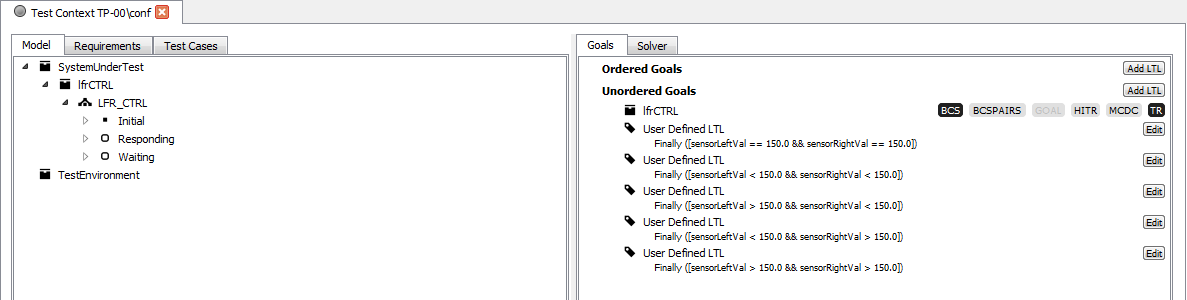
\includegraphics[width=1.0\textwidth]{lfr_mbtconf}
    \caption{Test Goal Configuration of LFR}
    \label{fig:lfr_mbtconf}
\end{figure}

\begin{figure}[htb!]
    \centering
	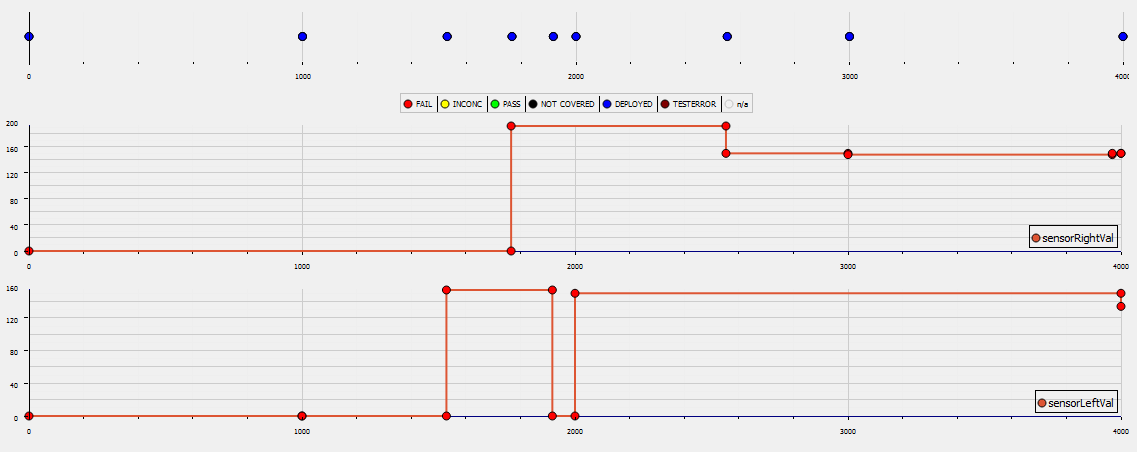
\includegraphics[width=1.0\textwidth]{lfr_input_seq}
    \caption{Test Input Sequence of LFR}
    \label{fig:lfr_test_seq}
\end{figure}

Firstly, the test result of \T{TP} against \T{Simulation} is displayed in Figure~\ref{fig:lfr_testcase_sum_sim}. All test cases should be \T{PASS} or \T{INCONCLUSIVE} because both \T{TP} and \T{Simulation} are test procedures generated from the exactly same test mode. However, three \T{FAIL}s are seen from the figure. This is because there is a very small delay in arrival time of inputs between \T{TP} and \T{Simulation}. For instance, $sensorLeftVal$ is changed to 150 from 0 at 2000 ms (as shown in Figure~\ref{fig:lfr_test_seq}) which is the time for \T{TP} to output it to \T{Simulation} as well as check of expected behaviour. But the actual time when \T{Simulation} gets the latest value 150 would be later (provided the Co-Simulation step is 1ms, and then there is 1ms delay). Finally, at 2000 ms, \T{TP} uses 150 to calculate the expected behaviour but \T{Simulation} still uses the old value 0 for $sensorLeftVal$ to give its output, which leads to mismatch of actual outputs with expected outputs. 
\begin{figure}[htb!]
    \centering
	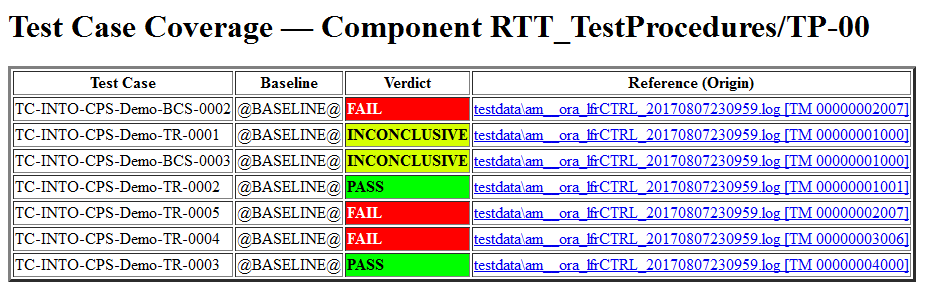
\includegraphics[width=1.0\textwidth]{lfr_sim_verdict}
    \caption{Test Case Summary (TP vs. SIM)}
    \label{fig:lfr_testcase_sum_sim}
\end{figure}

In order to correct it, we can put additional 2 ms offset manually in SUT. It is shown in the source code. Eventually, the test result of \T{TP} against \T{SUT} is displayed in Figure~\ref{fig:lfr_testcase_sum_sut} in which all test cases are \T{PASS} or \T{INCONCLUSIVE}.
\begin{figure}[htb!]
    \centering
	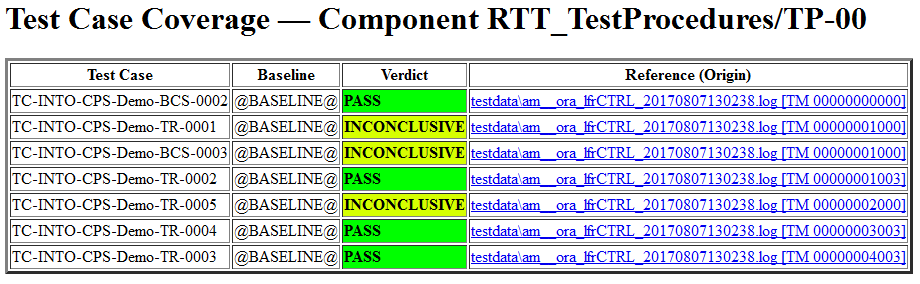
\includegraphics[width=1.0\textwidth]{lfr_sut_verdict}
    \caption{Test Case Summary (TP vs. SUT)}
    \label{fig:lfr_testcase_sum_sut}
\end{figure}

\subsubsection{Code Generation}

The VDM-RT model, \textbf{LFRController}, can be exported from Overture as a C code FMU, in addition to the tool wrapper FMU as used above. The \emph{LFRController-SourceCode.fmu} included in this pilot is obtained directly from Overture using the ``Export Source Code FMU'' option. However, this FMU does not contain binaries for co-simulation and so one may use the \emph{FMU Builder} included in the INTO-CPS Application to compile FMUs for Windows, Mac and Linux. 

This process has been performed and the resultant FMU is included in the pilot in the FMUs folder;  \emph{LFRController-Standalone.fmu}. One example experiment available is to switch this FMU for the tool wrapper version -- \emph{LFRController.fmu} -- and compare results. 
